

\chapter*{5 Results}
\label{results}
\addcontentsline{toc}{chapter}{5 Results}
\setcounter{chapter}{5}
\setcounter{section}{0}
\setcounter{figure}{0}
\setcounter{table}{0}

In this chapter the results of the autonomous system will be illustrated and discussed. Due to the two-part nature of the problem at hand, the results will be presented in accordance. This chapter does not aim to present new concepts, but simply illustrates the results of the complete system.

\section{Emulation results} 
\label{emuRes}
This section will detail the results obtained, when attempting to introduce basic LED flashing functionality, on the emulator as described in \textbf{\nameref{2emul}}. Firstly, it will be shown how the aforementioned functionality is achieved on a real-world MCU. Thereafter, the mentioned functionality will be demonstrated in an emulated environment.
\subsection{Real world MCU in STM32CubeIDE}
\label{real}

\begin{figure}[H]
\begin{center}
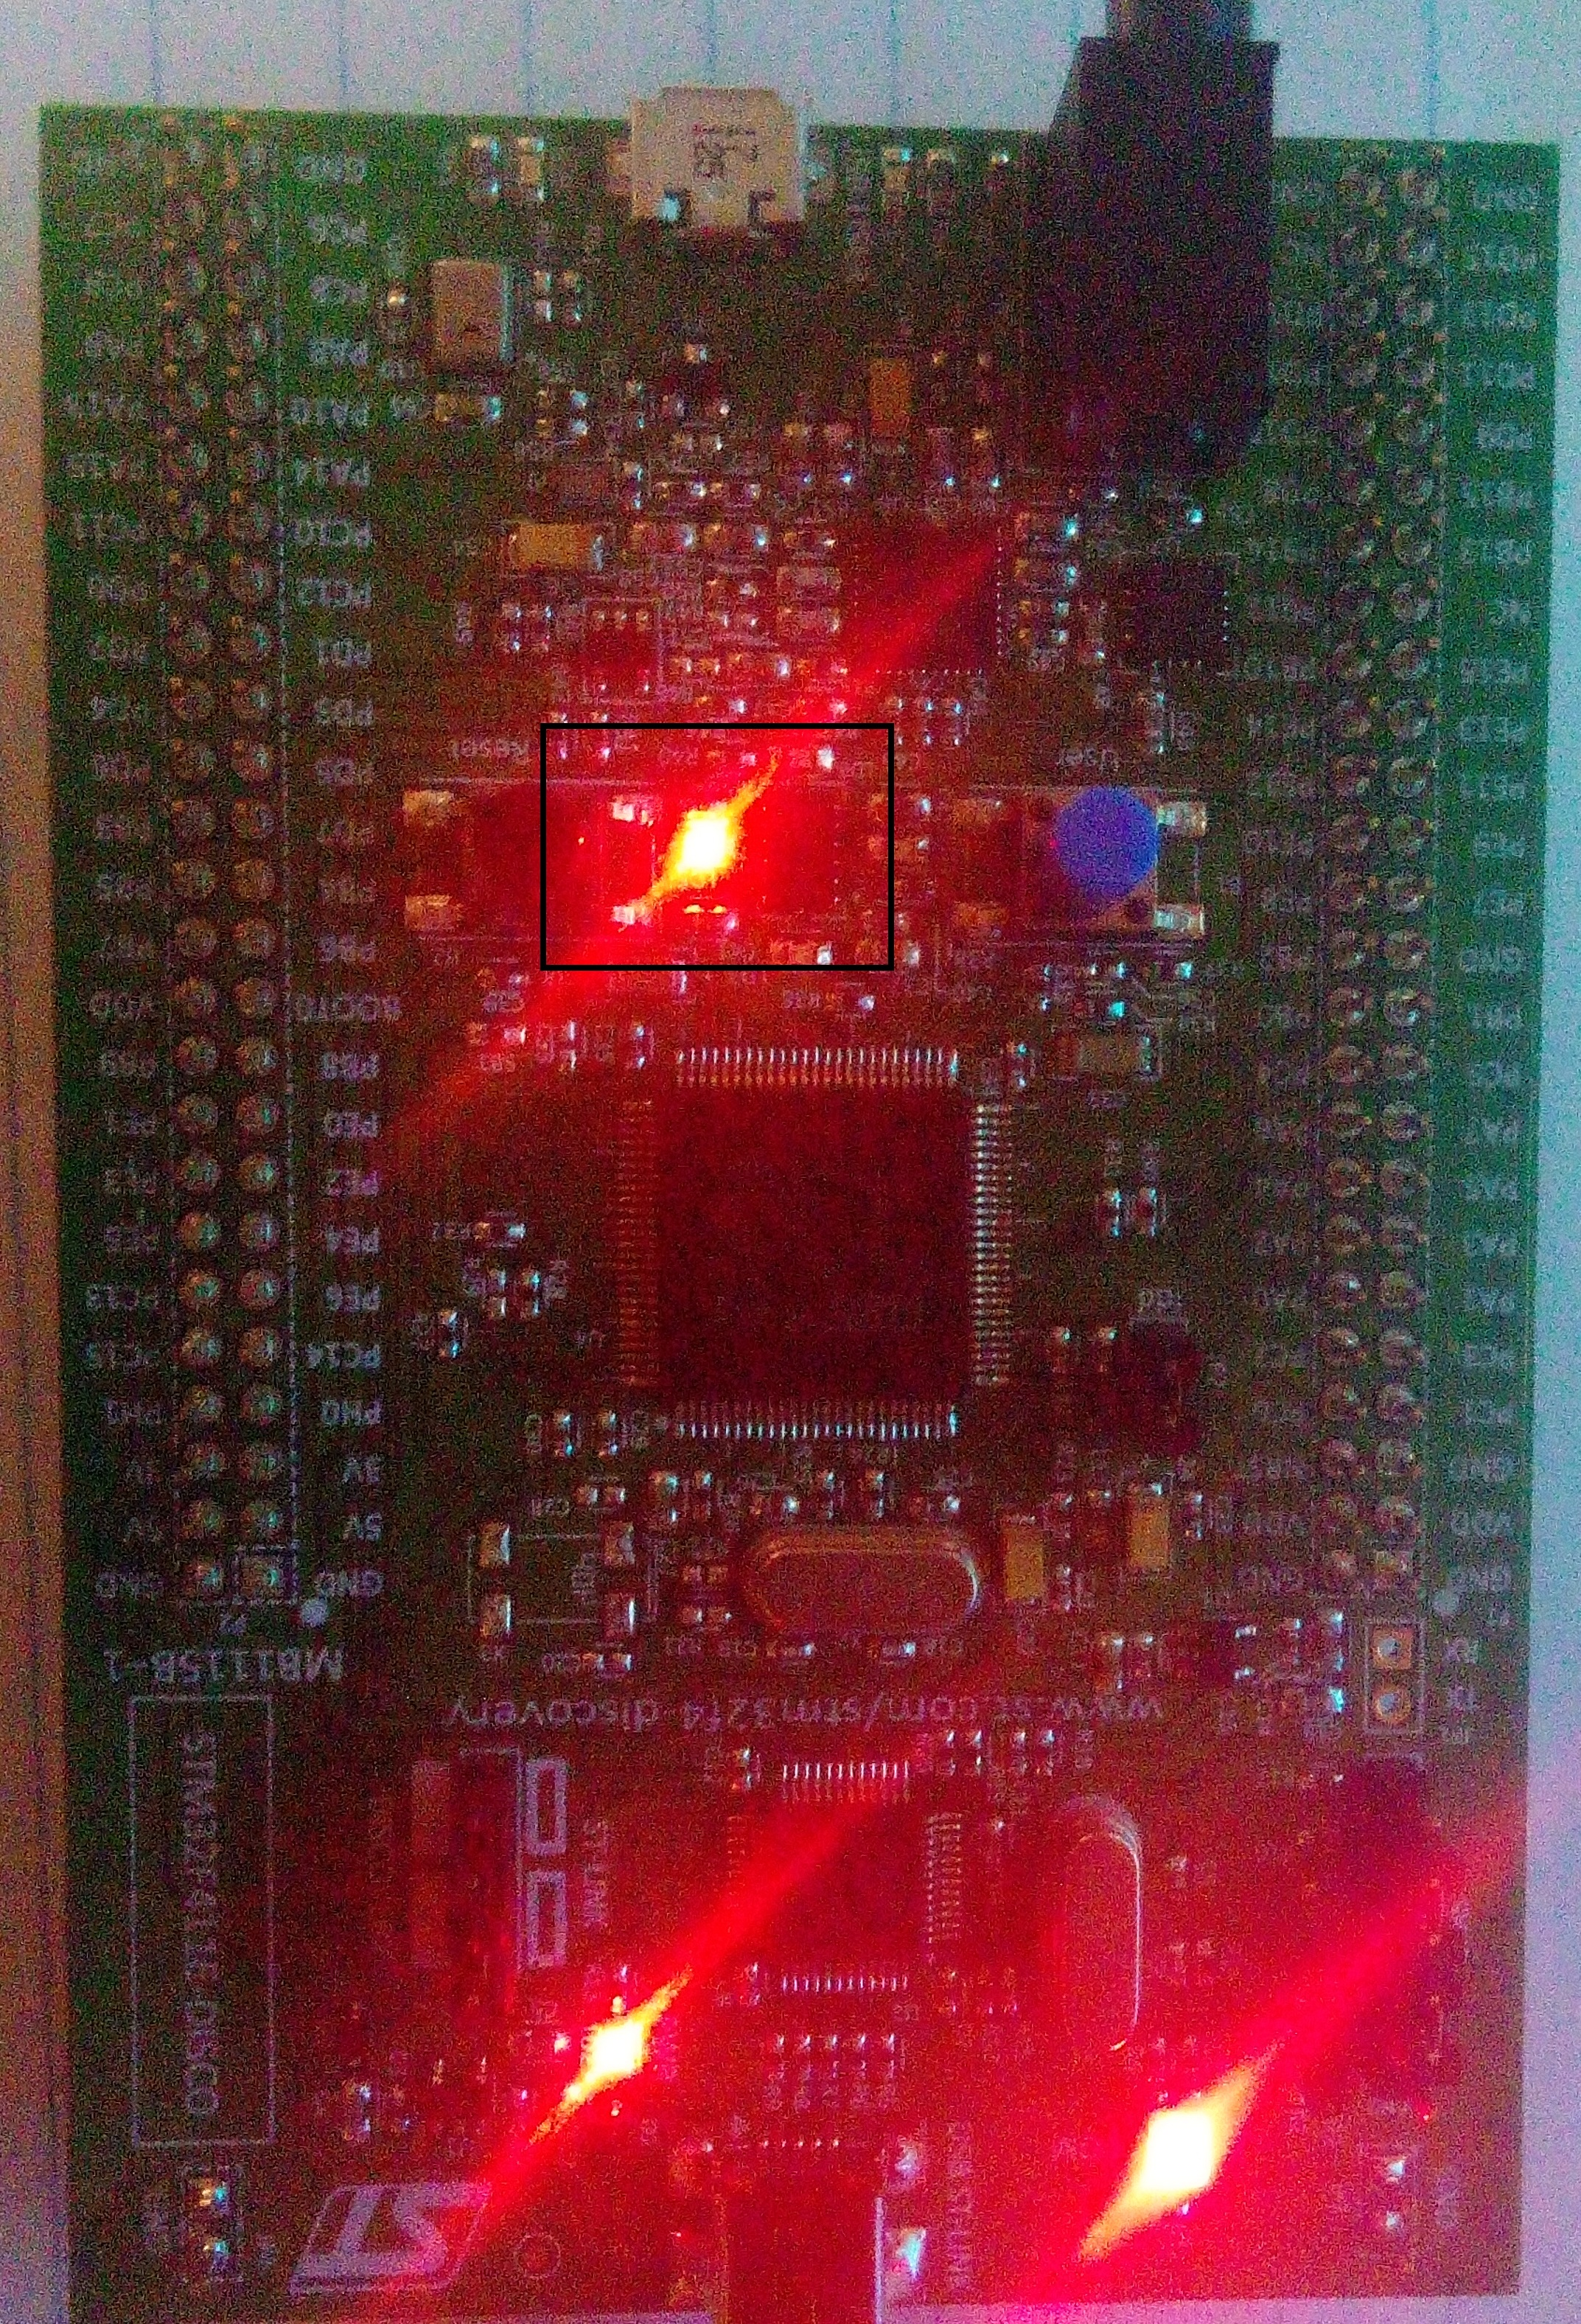
\includegraphics[width = 50mm, angle = 90]{re3.jpg}
\caption{Flashing red LED on real world MCU}
\label{re3.1}
\end{center}
\end{figure}

Figure~\ref{re3.1}, shows the blinking LED functionality on a real world MCU, namely the SMT32F411E. If this behaviour can be mimicked in the emulator, a promising solution to the problem in \textbf{\ref{ps} \nameref{ps}}, will have indeed been found.
\\\\
Figure~\ref{re3.2} illustrates the code required for the blinking of the red LED in STM32CubeIDE and can be viewed in the figure below.

\begin{figure}[H]
\begin{center}
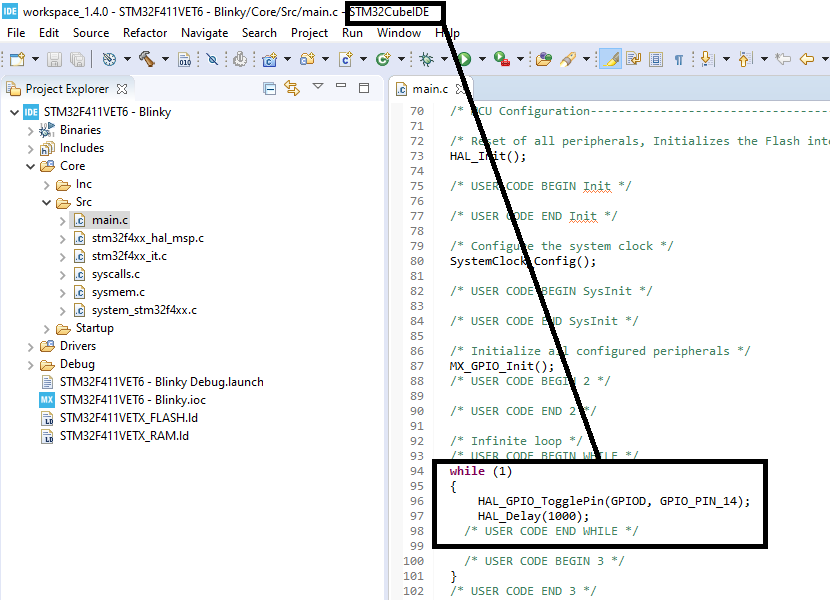
\includegraphics[width = 155mm]{re3.png}
\caption{Code in STM32CubeIDE to introduce LED blinking}
\label{re3.2}
\end{center}
\end{figure}




\subsection{Emulated MCU in Eclipse Embedded CDT}
\label{real}

\begin{figure}[H]
\begin{center}
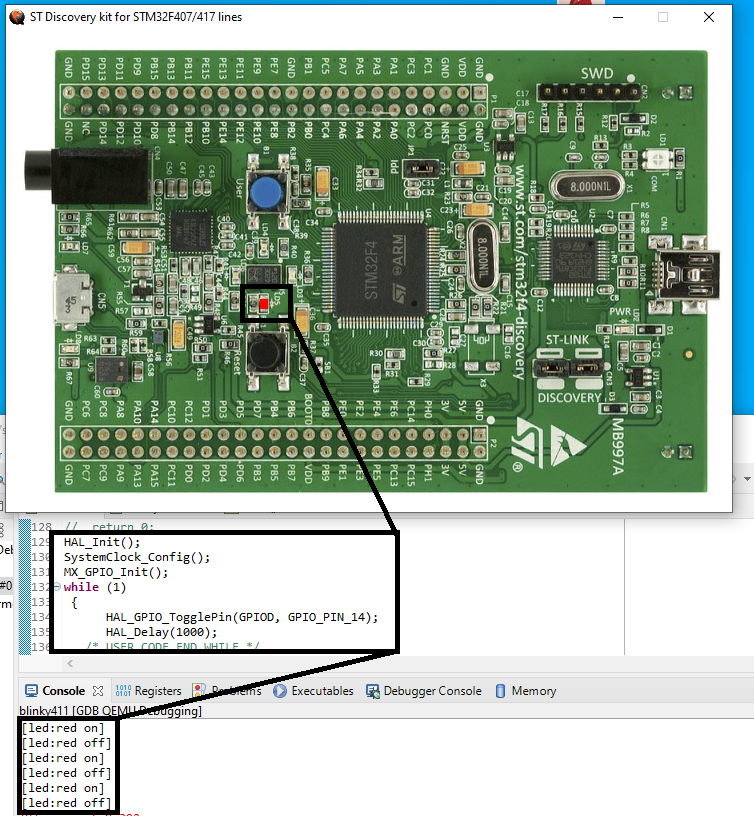
\includegraphics[width = 155mm]{re2.png}
\caption{Flashing red LED in emulated environment using code from STM32CubeIDE}
\label{re2}
\end{center}
\end{figure}

Figure~\ref{re2}, shows that the emulation process (using the same code as produced in STM32CubeIDE) is successful. The depicted basic functionality works on the emulator, despite it being a different MCU than the one used in STM32CubeIDE.

\section{Autonomous code evaluation results} 
\label{codRes}

The three step autonomous system was described extensively in \textbf{\nameref{4detailedd}}. In this section the results of the system will be illustrated.

\subsection{Step1 results}
\label{1res}

\begin{figure}[H]
\begin{center}
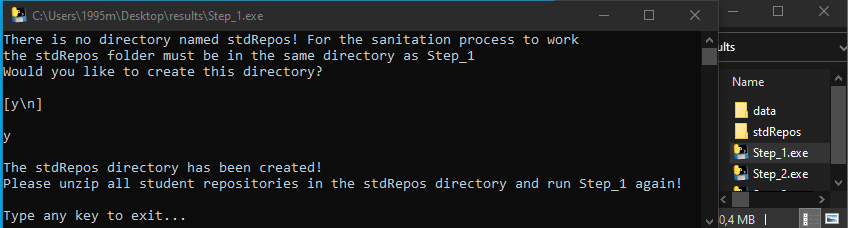
\includegraphics[width = 155mm]{r1.png}
\caption{Results after the first iteration of Step1}
\label{r1}
\end{center}
\end{figure}

Observable from Figure~\ref{r1}, is the state of the root directory (where the .py/.exe files are stored) after the first iteration of Step1.py/.exe. It can be seen that a terminal prompt appears requesting the user to create the "stdRepos" directory. Furthermore, the "data" directory is created within the program root directory. The user is instructed to unzip directories in the "stdRepos" folder.

\begin{figure}[H]
\begin{center}
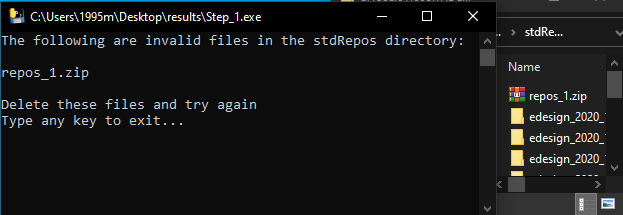
\includegraphics[width = 120mm]{r2.png}
\caption{Results after the second iteration of Step1}
\label{r2}
\end{center}
\end{figure}

Figure~\ref{r2}, displays the programs ability to detect unwanted files in the "stdRepos" directory. It can be observed that the required repositories have been unzipped, but the zipped file has not yet been deleted. The terminal prompts the user to do so and rerun Step1.py/.exe.

\begin{figure}[H]
\begin{center}
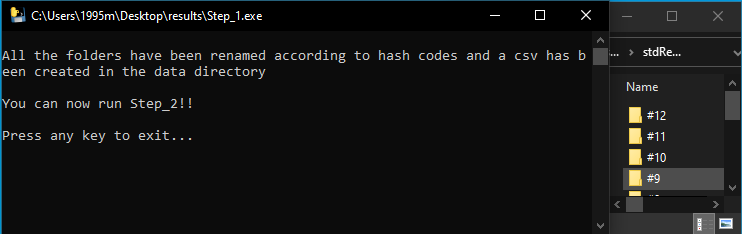
\includegraphics[width = 155mm]{r3.png}
\caption{Results after the third iteration of Step1}
\label{r3}
\end{center}
\end{figure}

Finally Figure~\ref{r3}, illustrates the renaming of the folder within the "stdRepos" directory in order to uphold anonymity as discussed previously. Furthermore, it can be seen that the terminal once again guides the user to the next step in the autonomous system.

\subsection{Step2 results}
\label{2res}

\begin{figure}[H]
\begin{center}
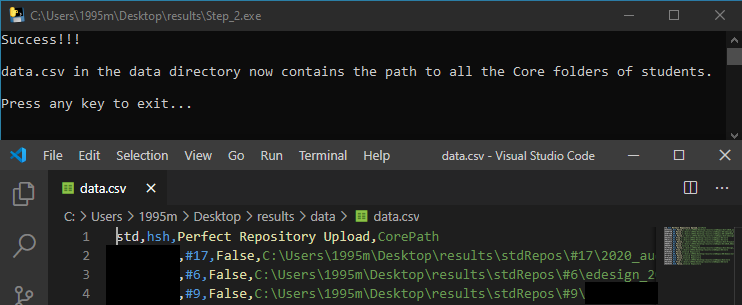
\includegraphics[width = 155mm]{r4.png}
\caption{Results after Step2}
\label{r4}
\end{center}
\end{figure}

Figure~\ref{r4} illustrates the state of the data.csv file within the "data" directory after the successful execution of Step2.py/.exe. It can be seen that the absolute path to the core folder is stored according to unique student identifiers. Student numbers in Figure~\ref{r4} have been censored for the sake of anonymity.

\subsection{Step3 results}
\label{3res}

\begin{figure}[H]
\begin{center}
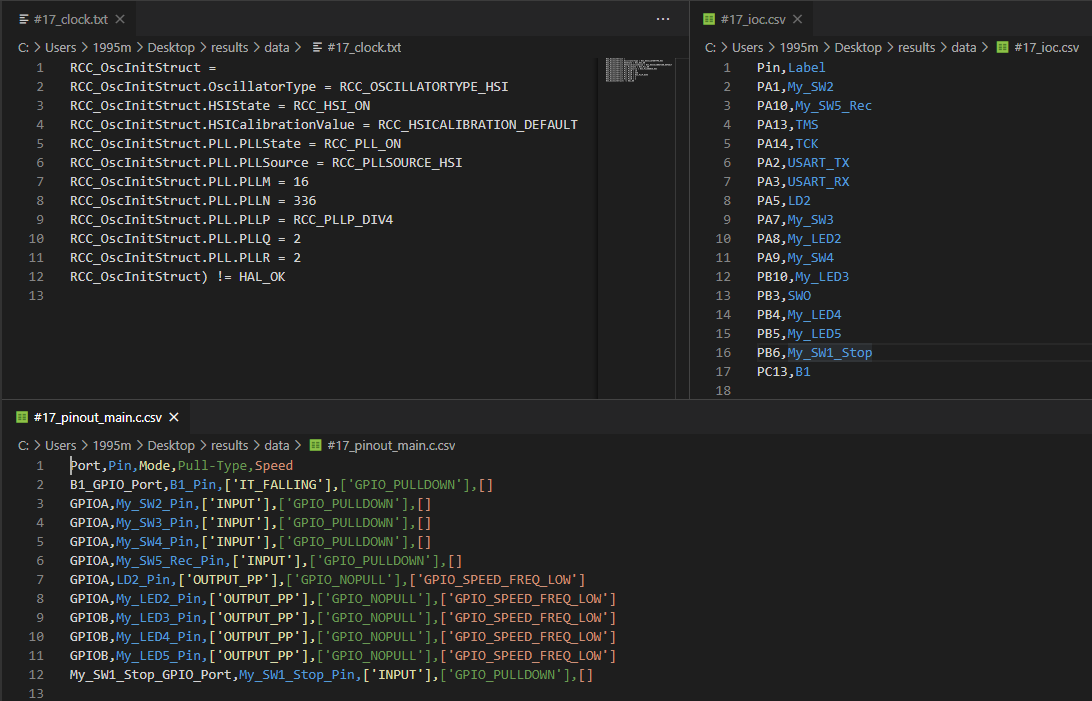
\includegraphics[width = 155mm]{r5.png}
\caption{Results after Step3}
\label{r5}
\end{center}
\end{figure}

The final step of the autonomous system produces the results depicted in Figure~\ref{r5}. The content of the three files outlined in \textbf{\ref{step3} \nameref{step3}}, are displayed for a specific student. It can be seen that the entire clock configuration is extracted and saved in addition to the pin configurations. It is, furthermore, observable that students often label pins within STM32CubeIDE. This makes it difficult to evaluate code, since pin numbers are not displayed in main.c when custom labels are applied. By extracting pin information from the .ioc files, however, the custom labels can be associated with specific pin numbers are seen in Figure~\ref{r5}.